\section{问题四的建模与求解：女胎异常判定}

\subsection{问题分析}

孕妇与女胎均不携带 Y 染色体，无法用 Y 浓度判断检测可靠性，需综合 X 染色体及 13/18/21 号染色体的 Z 值、GC 含量、读段数及相关比例、BMI 等因素判定女胎是否异常。以附件 AB 列（染色体非整倍体，空白即无异常）为判定结果标签，正常样本 537 例、异常样本 67 例，属类别不平衡的分类问题。

关键观察：仅用 ``$|Z|>3$'' 的单一阈值几乎无法识别异常（异常样本的对应染色体 Z 值并未系统性升高），说明女胎异常判定不能仅依赖单一染色体 Z 值，而需综合多维特征。

\subsection{判定方法}

本文采用两种监督分类模型并与临床 ``$|Z|>3$'' 基线对比。特征包括 13/18/21/X 染色体的 Z 值、X 染色体浓度、各染色体 GC 含量、原始读段数、唯一比对读段数、比对比例、重复读段比例、被过滤读段比例、GC 含量、年龄与 BMI 共 16 维。采用 5 折分层交叉验证评估，结果如表~\ref{tab:q4} 所示。

\begin{center}
\begin{tabular}{lccccc}
\toprule
\textbf{方法} & \textbf{准确率} & \textbf{灵敏度} & \textbf{特异度} & \textbf{F1} & \textbf{AUC} \\
\midrule
基线 $|Z|>3$ & 0.828 & 0.060 & 0.924 & 0.071 & 0.479 \\
逻辑回归 & 0.624 & 0.388 & 0.654 & 0.186 & 0.506 \\
随机森林 & \textbf{0.891} & 0.358 & \textbf{0.957} & \textbf{0.421} & \textbf{0.789} \\
\bottomrule
\end{tabular}
\captionof{table}{女胎异常判定模型对比（5 折交叉验证）}
\label{tab:q4}
\end{center}

随机森林综合多维特征后 AUC 达 0.789、特异度达 0.957，显著优于基线（AUC 0.479，接近随机）与逻辑回归，是较优的判定方法，体现了无创产前检测中结合测序质量指标与临床特征进行综合判定的优势\cite{ref3,ref6}。各模型 ROC 曲线如图~\ref{fig:q4_roc} 所示。

\begin{figure}[H]
  \centering
  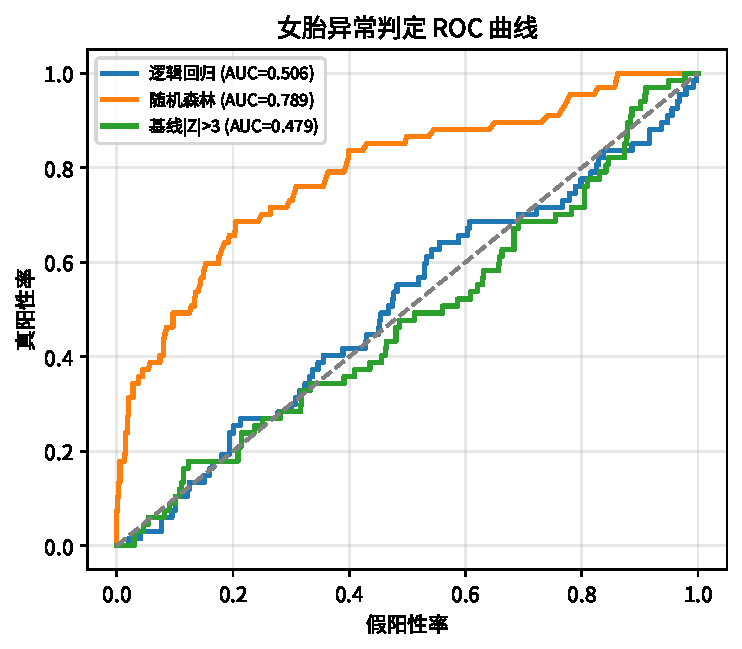
\includegraphics[width=0.62\textwidth]{../figures/fig4_1_roc.pdf}
  \caption{女胎异常判定 ROC 曲线对比}
  \label{fig:q4_roc}
\end{figure}

\subsection{特征重要性}

随机森林的特征重要性（图~\ref{fig:q4_imp}）显示，X 染色体浓度是最重要的判别特征（重要性 0.207），其次为各染色体 GC 含量、孕妇 BMI 与年龄。

\begin{figure}[H]
  \centering
  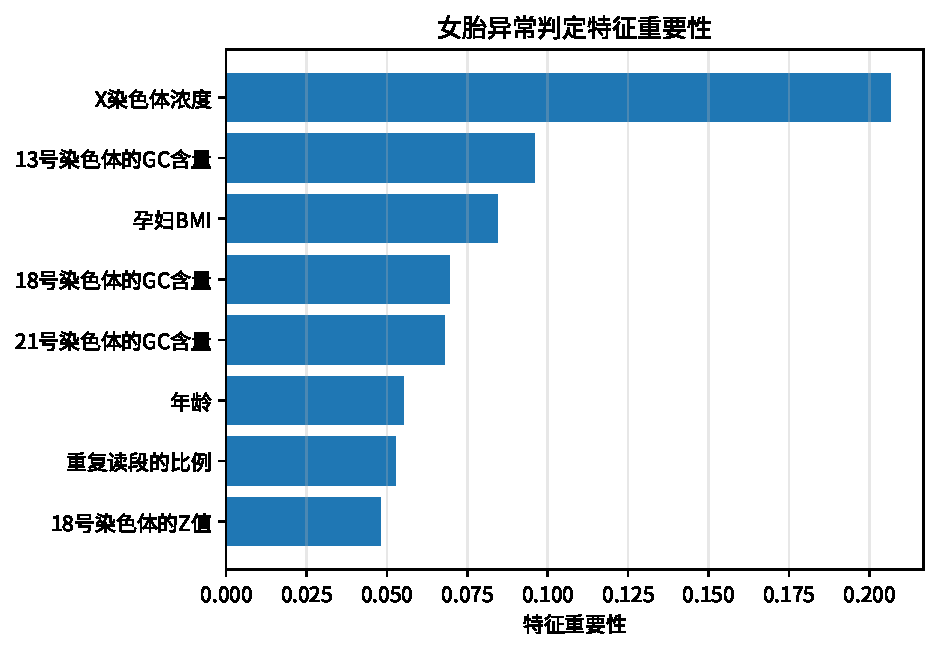
\includegraphics[width=0.62\textwidth]{../figures/fig4_2_feature_importance.pdf}
  \caption{女胎异常判定特征重要性}
  \label{fig:q4_imp}
\end{figure}

\begin{figure}[H]
  \centering
  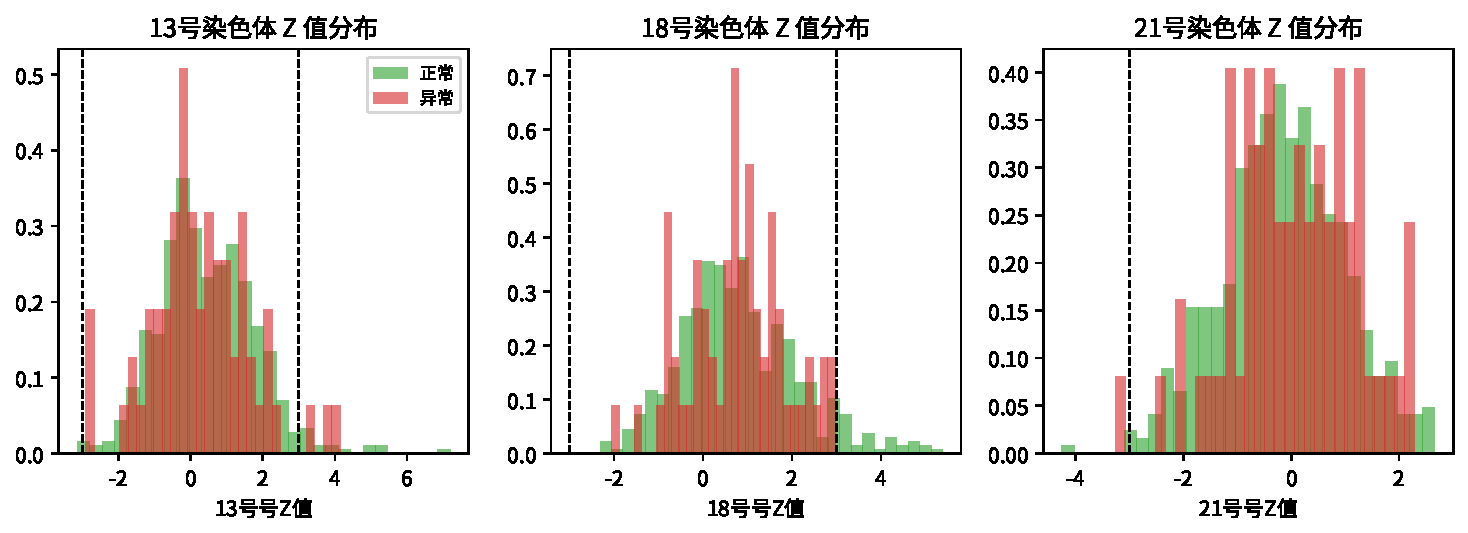
\includegraphics[width=0.9\textwidth]{../figures/fig4_3_z_distribution.pdf}
  \caption{正常与异常女胎在 13/18/21 号染色体 Z 值上的分布对比}
  \label{fig:q4_z}
\end{figure}

\begin{center}
\begin{tabular}{lcccccc}
\toprule
\textbf{特征} & X 浓度 & 13 号 GC & BMI & 18 号 GC & 21 号 GC & 年龄 \\
\midrule
\textbf{重要性} & 0.207 & 0.096 & 0.084 & 0.070 & 0.068 & 0.055 \\
\bottomrule
\end{tabular}
\captionof{table}{女胎异常判定特征重要性（Top 6）}
\label{tab:q4_imp}
\end{center}

由图~\ref{fig:q4_z} 可见，正常与异常女胎在单一染色体 Z 值上的分布高度重叠，印证了单一 Z 值阈值判定的失效；而 X 染色体浓度、GC 含量等质量指标蕴含更多判别信息。综上，本文给出女胎异常判定方法：以 X 染色体浓度、各染色体 Z 值、GC 含量、读段数及相关比例、BMI、年龄为特征，用随机森林模型输出异常概率，据此判定，较单一 Z 值阈值法显著提高判定能力。求解流程如图~\ref{fig:flow_q4} 所示。

\begin{figure}[H]
  \centering
  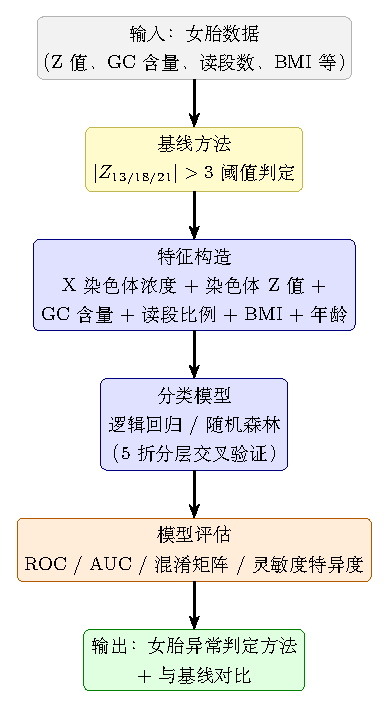
\includegraphics[width=0.72\textwidth]{../figures/fig_flow_q4.pdf}
  \caption{女胎异常判定流程}
  \label{fig:flow_q4}
\end{figure}
